\documentclass[12pt,a4]{article}
\newcommand{\evenfoot}{}
\usepackage{epsfig}
\usepackage{graphicx}
\usepackage{fancyhdr}
\usepackage{boxedminipage}
\usepackage{listings}
\usepackage{verbatim}
\usepackage{times}
\usepackage[latin1]{inputenc}
%\usepackage{ae}
%\usepackage{english}
%\usepackage{ngerman}
%\usepackage[german]{nomencl}
\usepackage[bookmarks, colorlinks=true, linkcolor=blue]{hyperref}
%\usepackage[bookmarks, colorlinks=false]{hyperref}

% set new Environment
\lstset{language=java}
%
% Texthoehe 46 Zeilen + \topskip
% (Rand ueber der Kopfzeile) : (Rand unter dem Text) = 1:2
%
\setlength{\textheight}{40\baselineskip}
\addtolength{\textheight}{\topskip}
\newlength{\uppermargin}
\setlength{\uppermargin}{\paperheight}
\addtolength{\uppermargin}{-\textheight}
\addtolength{\uppermargin}{-\headsep}
\addtolength{\uppermargin}{-\headheight}
\setlength{\uppermargin}{.333\uppermargin} % Raender oben/unten 1:2
\addtolength{\uppermargin}{-1in}
\setlength{\topmargin}{\uppermargin}
%
% Textbreite 5.2in
% Text hor. zentriert
%
\setlength{\textwidth}{5.2in}
\setlength{\oddsidemargin}{.5339in}
\setlength{\evensidemargin}{\oddsidemargin}
%
\pagestyle{headings}
\linespread{1.0}    % ein-zeilig
\linespread{1.6}    % zwei-zeilig
\linespread{1.3}    % eineinhalb-zeilig
%
\makeglossary
%
\begin{document}
%\title{Diplomarbeit}
%\author{Manfred Bergmann}
%\maketitle
% \sloppy	% damit beim trennen nix schief geht
% ----------------------------------------------------------------------------------
\begin{titlepage}
\begin{center}
{
	\large
    	\vspace{5.5cm}
    	\textbf{\Huge iKnow \& Manage} \\
    	\vspace{1cm}
    	User guide for iKnow \& Manage \\
    	\vspace{1cm}
    	Covers version 1.1 \\
    	\vspace{10cm}
}
    	Copyright by software by MABE\\
    	All right reserved \\
    	\href{http://www.software-by-mabe.com}{http://www.software-by-mabe.com} \\
    	\vspace{1cm}
	Document version 1.3 \\
    	\today
\end{center}
\end{titlepage}
% ----------------------------------------------------------------------------------
% ----------------------------------------------------------------------------------
\newpage
\tableofcontents
%\makeindex
% ----------------------------------------------------------------------------------
% ----------------------------------------------------------------------------------
\newpage
\section{Introduction}
\label{introduction}
\medskip
First of all, \textit{iKnow \& Manage} is a database system, like a knowledge database, capable of storing any kind of information. With its available datatypes (see chapter \ref{datatypes}) and the hierarchic organisation, you have absolute freedom in defining and specifying your data . \\
But storing the data is only one thing. Almost equal important is the search for data that you have brought into the system. With the search system of \textit{iKnow \& Manage} you are able to find for what you are searching. \\
For really private data that you want to store in the database like passwords or other data that nobody is allowed to read or to look at, you have the possibility of encrypting your data with a password you specified. \\
iKnow \& Manage also has a cute little text editor on board which you can use to write and store formatted texts. Or import, organize and watch your pictures with the integrated picture viewer. \\
The complete application uses drag \& drop. So it has been made easy to reorganise your data and/or to im-/ export data from other applications like the Mac OSX Finder and export data to other applications which are capable of drag \& drop respectively. \\
You can share your data with other users with the iKnow \& Manage archiv format that lets you export only the data you want to a file. With this you can do whatever you want, send your friend per eMail or save it on a backup disk. \\
\\
iKnow \& Manage is shareware. You are free to try the software and see whether it fits your needs for 30 days. If you decide to use it, you have to pay for it. A single user license costs US\$29.95. Limitations for an unregistered version are the main window that shows you are using an unregistered version in the window title, that is all. \\
If you want to register, see chapter \ref{registration} Registration on page \pageref{registration}.
% ----------------------------------------------------------------------------------
% ----------------------------------------------------------------------------------
\section{Getting started}
\label{getting_started}
\medskip
% ----------------------------------------------------------------------------------
\subsection{System Requirements}
\label{requirements}
\medskip
You should have a PPC or Intel Mac with at least Mac OSX 10.3.9 installed. \\
500 MBytes of RAM should be enough for the normal user. If you have a lot of data stored with this system some more RAM wouldn't hurt.
% ----------------------------------------------------------------------------------
\subsection{Installation}
\label{installation}
\medskip
Simply copy the ''iKnow \& Manage.app" that comes on the disk image somewhere on your hard disk and you are done.
% ----------------------------------------------------------------------------------
\subsection{How to read this guide}
\label{how_to_read}
\medskip
We thought it is not bad to know a bit of the base system before talking about all the windows, views and preferences that sometimes refers to the \textit{Datatypes} that are used in this system. \\
But you can read chapter \ref{gui} "User Interface" first if you want and cross reference to the appropriate "Datatype" in section \ref{datatypes}.
% ----------------------------------------------------------------------------------
% ----------------------------------------------------------------------------------
\newpage
\section{Datastore}
\label{datastore}
\medskip
iKnow \& Manage uses a small and efficient SQL database \\
(\href{http://www.sqlite.org}{SQLite}) for storing the data on your computer. But to achieve the dynamic and extendable content, an abstraction level has been added between the physical data and the data you see it in the application. See chapter \ref{gui_preferences} Preferences if you want to know more about the exact path that your data is saved.
% ----------------------------------------------------------------------------------
% ----------------------------------------------------------------------------------
\section{Datatypes}
\label{datatypes}
\medskip
To store data in the system you have some important datatypes available. Each has its purpose.
% ----------------------------------------------------------------------------------
\subsection{Items}
\label{items_datatype}
\medskip
\textit{Items} are some kind of collection or if you think of a table in a database or in a spreadsheet application they (if they do not have any subitems) are like a row where you can store other (none collection) datatypes (see next chapter for \textit{Values}). You even could say that Items are like objects. \\
However, if you nest Items you can build complete tables (then each nested Item is a row). But that is not all, with this you can even nest and build a hierarchy of complete tables. \\
That gives you the freedom of specifying the hierarchic data you might need. \\
\\
\textbf{Item Alias:} \\
An Item Alias is a special Item. It can not host any Values or subitems itself. It is only for referencing or cloning other Items. The only thing you have to do if you create an Alias is set the target the Alias should pint at. The target is a normal Item somewhere in the data hierarchy. Once you have set a target to the Alias (or you can just say "Create Alias" to one of your Items from the menu to have an Alias created and set with the target at once) you see that is has the same content as the target Item itself. If fact, if you alter any values of the Alias, they are altered to the original, too. \\
You can have as much Aliases in you system as you like.
% ----------------------------------------------------------------------------------
\subsection{Values}
\label{itemvalues_datatype}
\medskip
Now having a row, a table or simply a collection of data without data makes no sense. That's what \textit{Values} are for. \\
Values are used to fill the collections with data or to describe the objects or to specify data for the row and column of you table. \\
The system provides basic Values for you.
% ----------------------------------------------------------------------------------
\subsubsection{sText (simple text)}
\label{stext_datatype}
\medskip
Sometimes you have to store a text string, some words, or some sentences. Then this is the right Value choice. \\
If you have larger texts to edit or bring into the system you certainly are free to use the \textit{ExtendedText} (eText) type  where you can have formatted text.
% ----------------------------------------------------------------------------------
\subsubsection{Bool}
\label{bool_datatype}
\medskip
The Bool Value lets you specify the values 1 or 0, Yes or No, True or False.
% ----------------------------------------------------------------------------------
\subsubsection{Number}
\label{number_datatype}
\medskip
If you want to store any kind of number, the \textit{Number} Value is the right choice. \\
Since Numbers can be formatted in different ways (with thousands separator, number of decimal digits, ...) you are free to do so. \\
Specify the global Number format in Preferences (see Preferences in chapter \ref{gui_preferences} for more information) which is used as the standard format when a Number Value is new created. But you can change the format for each Number value as you wish.
% ----------------------------------------------------------------------------------
\subsubsection{Currency}
\label{currency_datatype}
\medskip
\textit{Currency} Values use the Number Values and extend them with a currency symbol. \\
As for Number Values you are free to choose the format of display for each Currency Value and additionally set a currency symbol for your Value.
% ----------------------------------------------------------------------------------
\subsubsection{Date}
\label{date_datatype}
\medskip
The \textit{Date} Value lets you specify Dates and Date ranges. \\
You also have the option so set an alarm. If the alarm date is due you are notified by a alarm window poping up. If you have Growl \href{http://growl.info/} installed you are also notified by Growl. 
% ----------------------------------------------------------------------------------
\subsubsection{URL}
\label{url_datatype}
\medskip
The \textit{URL} Value lets you specify URLs either on you local computer in form of any files or somewhere in the internet in form of Internet links. \\
\\
For the ones that do not know what an URL is exactly: \\
URL stands for (Uniform Resource Locator). URL is a standard for specifying resources, that is internet sites or other documents, that are stored somewhere on the internet or on your local computer. \\
Normally a URL looks like this: \\
\nolinkurl{http://www.software-by-mabe.com} \\ 
or \\ 
\nolinkurl{file://localhost/Users/manfred/Desktop/somefile.txt}  \\
(this at least on Unix system which Mac OSX is) \\
Every URL contains two distinct parts, the protocol specifier and the location specifier. Everything to here "://" is the protocol. In case of "http" it is the Hyper Text Transport Protocol. In the "file" case, you specify that this is a location on you local computer, a file. What comes after the ''://' is the location where to find the resource. In the first case it is in the WWW (World Wide Web) in the later case the location is a path to a local file. \\
Normally most software programs know what URLs are can handle them. So can this system. \\
\\
With this you can add resources or internet links to a object (Item) that you are describing or filling with data. \\
It even is possible to organise your complete internet link collection with this.
% ----------------------------------------------------------------------------------
\subsubsection{eText (extended text)}
\label{etext_datatype}
\medskip
We talked about the SimpleText Value which is for small texts without format. \\
Now if you need more text, formatted text you should choose the eText Value. \\
You have three different text format types available which are: \\
\\
TXT (plain text): is a normal text format. Actually I don't know if we can talk of a format here because with TXT you do not have much formatting possibilities (to be more precise, you have none). As plain text says, this is plain text. But this is very often wanted for a lot of purposes. For example if you are an internet developer you know that you best save your HTML source code as plain text, because otherwise the browser would have difficulties parsing the formatted text file and display you site. Or for me as software developer, we save our source code text files files as plain text. Because no compiler will parse formatted text. \\
\\
RTF (Rich Text Format): this format is known by almost every word processor application and is with that highly distributable and platform independent. RTF is capable of storing images within the document and much more. RTF is the default selected format if you open the "TextEdit" application on you Mac. \\
\\
RTFD (Rich Text Format Directory): RTFD is the successor of RTF but it is not so widespread and known to other word processor applications like RTF is. So this format might only be used on Mac systems. \\
\\ 
eText Values are special values because they may not be stored in our database directly. All have the possibility to link (refer) to an existing file outside of our database e.g. on you filesystem or on the internet. The data then is not stored in our database directly but at the location you specified. \\
Example: you have a text document somewhere on the internet, that you are maintaining and at the same time proving to others. You can edit the document, read and save directly on this location without explicitly "downloading" or "uploading" it from or to the internet. This is described in chapter \ref{bring_data} "Bringing data into the system".
% ----------------------------------------------------------------------------------
\subsubsection{Image}
\label{image_datatype}
\medskip
The \textit{Image} Value is mainly a type used for storing pictures or image data within an Item. Included with this applications is a small picture viewer that can show these images. You cannot create or edit Images here. \\
You also can choose to import the complete image data into the database or only refer to it through a URL somewhere in the internet or on your local computer.
% ----------------------------------------------------------------------------------
\subsubsection{File}
\label{file_datatype}
\medskip
The \textit{File} Value is for all other types of file data that you need. The same is true here as for Image and eText values. You can import the file data or refer to it. That is your choice. \\
% ----------------------------------------------------------------------------------
\subsubsection{Value Alias}
\label{itemvalueref_datatype}
\medskip
A \textit{Value Alias} is mostly the same as the Item Alias. You can refer to any Value in the system. And altering the reference alters the original as well. To create one either choose "Create Alias" from the menu or create an empty Value Alias and set the target manually.
% ----------------------------------------------------------------------------------
\subsection{System-Items}
\label{systemitems_datatype}
\medskip
There are some Items that you cannot delete or edit (see next chapter). They almost all are in the root hierarchy.
% ----------------------------------------------------------------------------------
\subsubsection{Templates}
\label{templates_systemitem}
\medskip
Any Item that you have created can be used as template. Simply copy \& paste or drag \& drop an Item to the Templates System-Item and it will be available through the menu is you want to add a new Item. Additionally you can choose "Define as Template" from the main menu or context menu to define any Item as a template Item. \\
All Items that are on the first level under the Templates Item are Template Items. You can create new Items from these templates by choosing "From Template" in the main menu or from the context menu.
% ----------------------------------------------------------------------------------
\subsubsection{Imports}
\label{imports_systemitem}
\medskip
All external data (e.g. files, images, ...) that you drop onto the application icon go to Import System-Item.
Additionally, if you choose "Import..." from the main menu or context menu and import external data to iKnow \& Manage and you don't have a Item selected as destination for the import. The data goes to Imports, too.
% ----------------------------------------------------------------------------------
\subsection{The IKAM Archiv}
\label{ikam_archiv}
\medskip
iKnow \& Manage has it's own file format for importing and exporting data (see chapter \ref{bring_data} "Bringing data into the system" and chapter \ref{export_data} "Exporting data" for more information on that). You can use it to export or import (to or from file) whole subtrees of you data. This is quite nice if you want to make individual backups or simply send it to someone else per eMail. \\
The IKAM-Archiv file has the file extension "ikam".
% ----------------------------------------------------------------------------------
% ----------------------------------------------------------------------------------
\newpage
\section{Bringing data into the system}
\label{bring_data}
\medskip
Normally you create new Items or Values with selecting the "Add Item" or "Add Value" menu or toolbar functions. You then can fill them with data.
% ----------------------------------------------------------------------------------
\subsection{Entering simple data}
\label{enter_simple_import}
\medskip
Most Values provide text input fields where you can easily enter text. Even for Number and Currency Values you enter the number value as text. For Date Values there are date picker controls that help you entering or setting a date. Off course you can enter the date by hand if you want to.
% ----------------------------------------------------------------------------------
\subsection{Copy \& Paste}
\label{cp_import}
\medskip
Copy \& Paste is available in the whole system. You can copy complete Items or Values to the pasteboard and paste them somewhere else in your data hierarchy. You also can copy parts of text documents in an other application and paste the text in a text input field of a sText or eText Value (or the other way round).
% ----------------------------------------------------------------------------------
\subsection{Drag \& Drop}
\label{dd_import}
\medskip
We distinguish between internal drag \& drop and external drag \& drop. \\
\emph{Internal} d\&d is used for reorganising your Item hierarchy or for moving/copying Items and Values from one location to another. \\
\emph{External} d\&d is used for exporting and importing data (to and from the application outside world). \\
To import a file from the Finder, drag a file and drop it somewhere in the application or on the application icon (this import goes to Imports, we talked about it). The type of Value that is created with this operation cat be set up in the Preferences dialog. Normally Image files are created as Image Values, text files that have the ending ".txt", ".rtf", ".rtfd" are normally imported as eText Values. All file extension known to iKnow \& Manage can be set in the preferences. \\
If a file is an IKAM-Archiv (see chapter \ref{ikam_archiv} "The IKAM-Archiv") it is treated like that and the system tries to import the exported IKAM-Archiv with all its Items and Values. \\
URLs from other applications like E-Mail programs or web browsers can simply be dropped onto iKnow \& Manage, too. With this a URL Value should be created.
% ----------------------------------------------------------------------------------
\subsection{Manual Import}
\label{manual_import}
\medskip
The same imports that you can do with drag \& drop you can do manually, too. Simply choose "Import..." from the main menu or the context menu. \\
The import settings are taken from the default settings set in preferences, but on manual import you can override these settings in the requester that appears when you choose this menu action.
% ----------------------------------------------------------------------------------
% ----------------------------------------------------------------------------------
\newpage
\section{Exporting data}
\label{export_data}
\medskip
Now, that we have talked about importing data. It is important to talk about exporting your data. \\
Sometimes it is necessary to export some data, because you may want to make backups of subtrees of your data to store them somewhere on the net or on your computer.
% ----------------------------------------------------------------------------------
\subsection{Copy \& Paste}
\label{cp_export}
\medskip
Generally all your data can be exported with copy and paste. But since the simpler Value types like Number, Currency, Date, Bool and the Items itself are stored in a proprietary format (IKAM format), it is unlikely that other applications can use this data that has been copied to the pasteboard. All other Values are copied not only as IKAM format to the pasteboard. Texts are copied as texts, URL are copied as URLs, Images are copied as Images. Applications that do accept these types can import them.
% ----------------------------------------------------------------------------------
\subsection{Drag \& Drop}
\label{dd_export}
\medskip
Almost the same that is true for copy \& paste is true for drag \& drop. The data is treated is the same way. The difference here is, that you can set default export settings for drag \& drop in the preferences. Since you won't get a requester if you for instance drop an Image Value to the Finder, the system has to know which export format you prefer.
% ----------------------------------------------------------------------------------
\subsection{Manual Export}
\label{manual_export}
\medskip
The manual export function uses the same export functions as the drag \& drop export. But, you have to trigger the export action by choosing "Export..." from the main menu or from the context menu. And here you will be prompted to set a file or directory to export your data to. Additionally, you explicitly can choose which export type you want to use. These setting are taken from the preferences, but you can override them. \\
Both the integrated text editor for eText Values and the integrated image viewer have the possibility of saving the text or the image to a path on you hard disk.
% ----------------------------------------------------------------------------------
\subsection{Indirect Export}
\label{indirect_export}
\medskip
Some Values can be opened in the standard application for this type or in an application by your choice. This can be done by pressing the "Open" or "Open with..." button in the "Details" tab on a open "Information" (see chapter \ref{gui_information} "Information View") drawer. So the data gets exported here and imported by another application.
% ----------------------------------------------------------------------------------
\subsection{HTML Export}
\label{html_export}
\medskip
You can export single Values or complete Items as HTML lists. If you choose one or more Items to export you will get an HTML list for each Item with all its Values. If you need more detailed lists, you should choose one or more Values and export them as HTML. Texts from ExtendedText Values are displayed inline and are additionally copied to the export folder. The thumbnail pictures of Image Values are also displayed.
% ----------------------------------------------------------------------------------
% ----------------------------------------------------------------------------------
\newpage
\section{User Interface}
\label{gui}
\medskip
% ----------------------------------------------------------------------------------
\subsection{Main Window}
\label{gui_mainwindow}
\medskip
On the main screen (figure \ref{image:startup}) you can see the main parts of the application. That is the toolbar with its buttons on the top, the Item tree view on the left side, the Value list view on the right. \\
Now, if you choose an Item on the left, you will see all its Values on the right side. Pretty simple.
% 
\begin{figure}[ht]
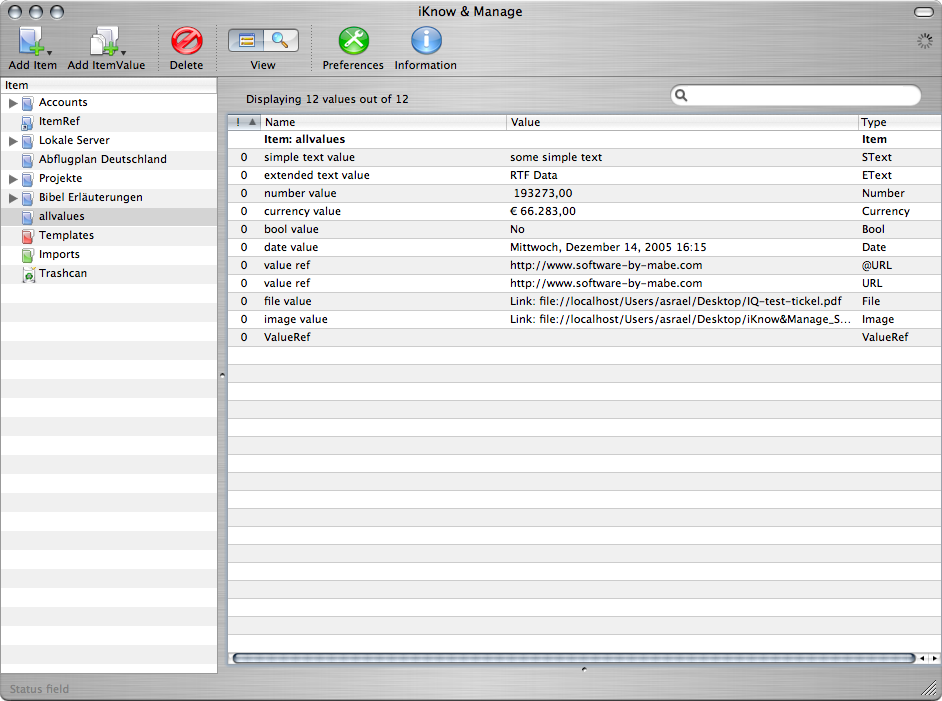
\includegraphics[width=13.5cm]{images/MainWindow.png}
\caption{Startup screen}
\label{image:startup}
\end{figure}
\noindent
% ----------------------------------------------------------------------------------
\subsection{Toolbar}
\label{gui_toolbar}
\medskip
Some functions of the application are available through a button in the toolbar (see figure \ref{image:toolbar}). Adding new Items, adding new Values to the current selected Item, deleting the current selection, either Items or Values, that depends on which view is the active one. If you last selected one or more Values and choose delete, then the selected Values are deleted although an Item is also highlighted in the Item tree view. \\
The application provides a separate view for searching which can be selected with the \textit{View} toolbar item. \\
The \textit{Preferences} brings up the preferences dialog window which is described later in chapter \ref{gui_preferences}. \\
For more information (see chapter \ref{gui_information} \textit{Information View} later) on Items or Values you should open the information panel or drawer with the information toolbar button.
% 
\begin{figure}[ht]

\includegraphics[width=13.5cm]{images/Toolbar_shot.png}
\caption{Toolbar}
\label{image:toolbar}
\end{figure}
\noindent
% ----------------------------------------------------------------------------------
\subsection{Item tree view}
\label{gui_itemoutlineview}
\medskip
% 
\begin{figure}[ht]
\begin{center}
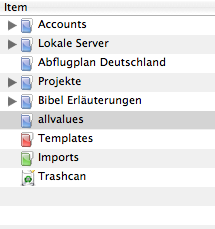
\includegraphics[width=5.0cm]{images/OutlineItemView.png}
\end{center}
\caption{Item Treeview}
\label{image:itemoutlineview}
\end{figure}
\noindent
%
The main data tree is located on the left of the main window. It is displayed with a tree view component. Here you build your hierarchical data structure of Items. \\
Add new Items either through the toolbar menu or right click with your mouse in the tree view and choose to add a new Item.
% ----------------------------------------------------------------------------------
\subsection{Value list view}
\label{gui_itemvaluelistview}
\medskip
% 
\begin{figure}[ht]
\begin{center}
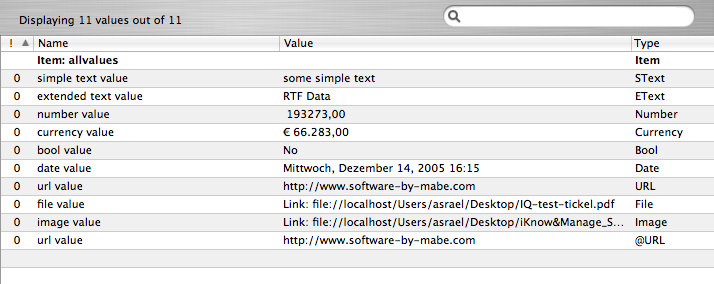
\includegraphics[width=13.5cm]{images/ItemValueListView.png}
\end{center}
\caption{ItemValue Listview}
\label{image:itemvaluelistview}
\end{figure}
\noindent
%
In this view you see all Values that a (or more) selected Item has. As you can see in figure \ref{image:itemvaluelistview} this can be any kind of Value. \\
If you do a right click with your mouse you get a context menu. \\
\\
Above the list view itself is a text input field, a \textit{search field}. If you enter something here, the Values are filtered and only the ones that \textit{match} the string you entered are displayed. All Values of every selected Item are filtered as long as a string is in the search field. \\
The list view has four columns. The first is the \textit{sortorder} column. Here you can set an integer value that you can use to individually sort your Values. The second column is the \textit{name} of the Value. It can be altered either with double clicking in the cell or with the information view (is described later, see chapter \ref{gui_information}). The third column is the \textit{value} of the Value itself which you can edit for the simple Values (sText, Number, Currency, Date, URL) in the list view itself. For more complex Values (eText, Image, File) you have to use the information view. The fourth column displays the type of the Value.
% ----------------------------------------------------------------------------------
\subsection{Information View}
\label{gui_information}
\medskip
% 
\begin{figure}[ht]
\begin{center}
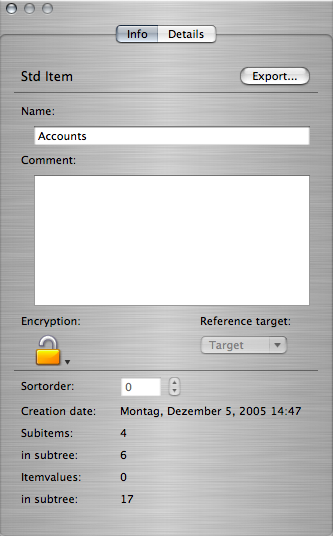
\includegraphics[width=6.0cm]{images/Item_InfoView.png}
\end{center}
\caption{Item Infoview}
\label{image:iteminfoview}
\end{figure}
\noindent
%
An additional \textit{Information} panel (or drawer, depends what you selected in preferences) opens and shows either information or details of the current selected Item or Value. You can switch between \textit{Info} and \textit{Details} simply by clicking on the tab. \\
The Info tab show information for both Item and Value (whichever you have selected). Here you can change the name of the selection and write a comment. Encrypting, decrypting and changing the sortorder is only available for Values. \\
Some additional information like when this Item has been created, how many Subitems it has and how many Values it has is shown below. \\
If the selection is a Item or Value Alias you can set the target (the target of the alias) with the pop up button "Reference Target". \\
This view also has a \textit{Export} button which lets you export the current Item or Value either as IKAM-Archiv or as its native type (see chapter \ref{manual_export} for more information of this).
% ----------------------------------------------------------------------------------
\subsection{Detail View}
\label{gui_detailview}
\medskip
We cover here only the detail views of the complex Values because all other Values should be easy to handle. Most of the information is the same for all three Values and their detail views. \\
For all complex Values (eText, Image, File) you can choose if you want the data to be saved in the \textit{internal} database or if you want to save the it \textit{externally} with linking to a file in the file system. \\
The eText Value is a bit different from the other two in that you can create the text document with the build-in text editor. So whenever you create a new eText Value you can begin to write your text immediately in the editor and the data is per default saved in the internal database. \\
If you want to import a text document and do not need the file anymore, just switch to \textit{Internal} and press the \textit{import} button. A file requester will appear and you can choose the file to be imported. If you want to link to an external File, switch to \textit{External} and either choose the the file with the \textit{Path} button or set an URL in the Path/URL text field above. Here you also can enter an URL that is somewhere in the internet or in your local network. You also have the option of choosing an already defined URL Value somewhere in you data hierarchy. The \textit{URLs} pop up button lists all URL Values that are available in the system (that you have entered) and you can choose one here. Once you have entered a link value for the external file you will see informations about this URL, is it \textit{valid}, is it a \textit{local} URL and is it \textit{connectable}. The selection between internal and external and choosing/editing the external link URL is the same for all three complex Values. \\
Since the documents you might refer to can be bigger in size, you have the possibility of loading the data every time you select the Value (\textit{Auto load} activated) or you load them manually when I need you (\textit{Auto load} deactivated). \\
The \textit{Open} button opens the data with the standard defined application for this type. The \textit{Open with...} button lets you choose the application to open the data with.
% ----------------------------------------------------------------------------------
\subsubsection{eText Info View}
\label{gui_etext_info}
\medskip
% 
\begin{figure}[ht]
\begin{center}
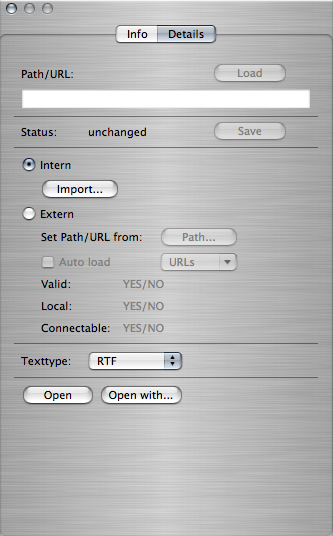
\includegraphics[width=6.0cm]{images/ItemValue_EText_DetailView.png}
\end{center}
\caption{ItemValue eText Detailview}
\label{image:itemvalueetextdetail}
\end{figure}
\noindent
%
Choose the \textit{Texttype} with the pop up button. The format that has been selected here is used to save the data. If you choose \textit{TXT} your text data is saved as plain text, if you choose \textit{RTF} you data is saved as RTF data. See chapter \ref{etext_datatype} for more information on eText Values and formats.
% ----------------------------------------------------------------------------------
\subsubsection{Image Info View}
\label{gui_image_info}
\medskip
% 
\begin{figure}[ht]
\begin{center}
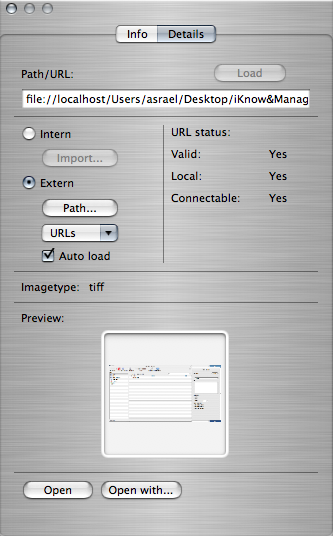
\includegraphics[width=6.0cm]{images/ItemValue_Image_DetailView.png}
\end{center}
\caption{ItemValue Image Detailview}
\label{image:itemvalueimagedetail}
\end{figure}
\noindent
%
The image detail view shown most of the information the eText details view also does but additionally it has information about the image, size, type, ... and also an preview.
% ----------------------------------------------------------------------------------
\subsubsection{File Info View}
\label{gui_file_info}
\medskip
% 
\begin{figure}[ht]
\begin{center}
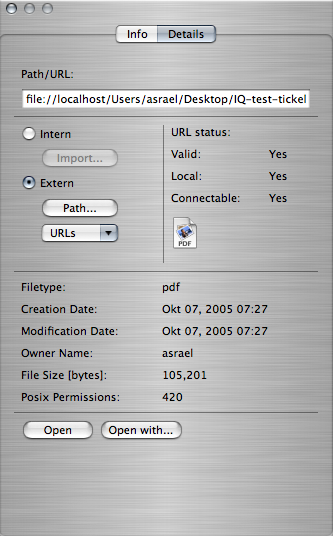
\includegraphics[width=6.0cm]{images/ItemValue_File_DetailView.png}
\end{center}
\caption{ItemValue File Detailview}
\label{image:itemvaluefiledetail}
\end{figure}
\noindent
%
In contrast to the eText and Image Values which are special in their usage, the File Value is for all other files you might use and want to import into the application. The details view shows the file icon and some other information of the file like owner and file size and so on (only if linked from local hard drive or when imported).
% ----------------------------------------------------------------------------------
\subsection{Search View}
\label{gui_search}
\medskip
% 
\begin{figure}[ht]
\begin{center}
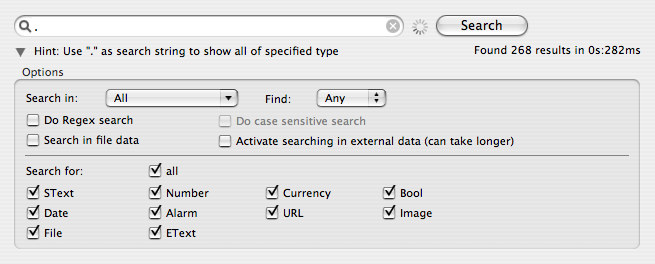
\includegraphics[width=13.5cm]{images/Search_View.png}
\end{center}
\caption{Search View}
\label{image:searchview}
\end{figure}
\noindent
%
Despite the search text field in the Value list view that was more or less only a filter, this one here searches the complete database for the search string you've entered. Simply enter a search string into the search text field and press enter or click on the search button. Searching all data could possibly take some seconds. \\
You can also choose to search in a special Item. Default setting is searching in "all" Items. \\
\\
You also have the possibility to define which type of Value you are searching for. Simply check or uncheck one or more of the type checkboxes in the search options. \\
For people knowing about regular expressions. If you check this, the string entered in the search text field is treated as regular expression.
% ----------------------------------------------------------------------------------
\subsection{Integrated text editor}
\label{gui_texteditor}
\medskip
The integrated text editor is for eText Values. Once you created such a Value, and you select it, the text editor is shown and awaits your input. Please set the right text type in the eText Info View (see chapter \ref{gui_etext_info}). The rulers can be activated with the corresponding checkbox. But they only are available for RTF and RTFD texts. Plain TXTs cannot have rulers. \\
Spell checking can be activated for all text types. \\
If you hit the "Save" button (alternatively you can press <Apple>-S), the text is saved to the location where it has been loaded from. With hitting the "Save as" button a requester pops up and lets you choose the save location and the text type for saving. \\
For formatted texts you can set another color or font with the color and font panes accessible through the buttons.
% 
\begin{figure}[ht]
\begin{center}
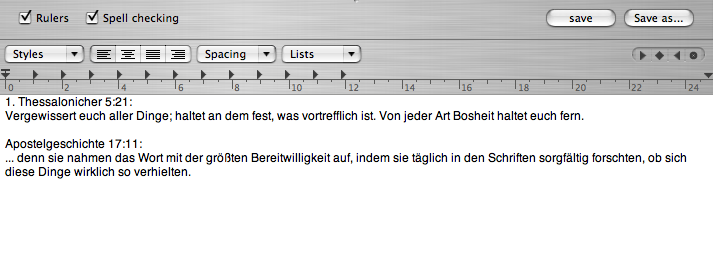
\includegraphics[width=13.5cm]{images/Editor_View.png}
\end{center}
\caption{Text-Editor}
\label{image:texteditor}
\end{figure}
\noindent
%
% ----------------------------------------------------------------------------------
\subsection{Integrated image viewer}
\label{gui_imageviewer}
\medskip
The integrated image viewer has two scaling methods, selectable through the pop up button on the left (see figure \ref{image:imageviewer_scaletofit}). \textit{ScaleToFit} always tries to scale the image to fit in the space that is available. With \textit{ManualScale} (see figure \ref{image:imageviewer_manualscale}) the scaling controls are activated and you can scale yourself. The maximum zoom is 200\%. \\
The "Save as" button lets you save the image to a location and additionally you can choose a image type to save. 
% 
\begin{figure}[ht]
\begin{center}
\includegraphics[width=13.5cm]{images/ImageViewer_View_ScaleToFit.png}
\end{center}
\caption{ImageViewer Control ScaleToFit}
\label{image:imageviewer_scaletofit}
\end{figure}
\noindent
%
% 
\begin{figure}[ht]
\begin{center}
\includegraphics[width=13.5cm]{images/ImageViewer_View_ManScale.png}
\end{center}
\caption{ImageViewer Control Manual Scale}
\label{image:imageviewer_manualscale}
\end{figure}
\noindent

% ----------------------------------------------------------------------------------
\subsection{Preferences}
\label{gui_preferences}
\medskip
% ----------------------------------------------------------------------------------
\subsubsection{General}
\label{prefs_general}
\medskip
% 
\begin{figure}[ht]
\begin{center}
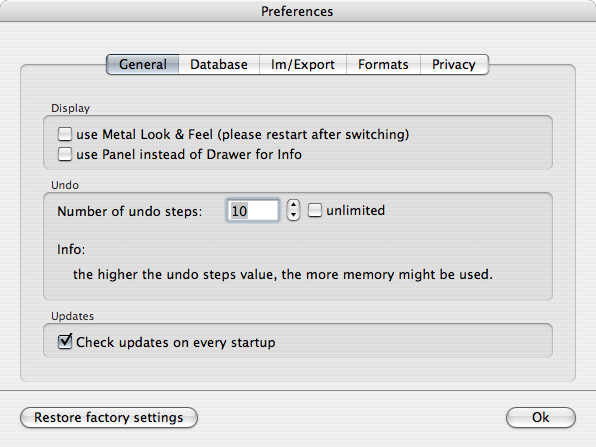
\includegraphics[width=13.5cm]{images/Prefs_General.png}
\end{center}
\caption{General Prefs}
\label{image:generalprefs}
\end{figure}
\noindent
%
In the general prefs you can choose if you want to have Brushed Metal or Aqua Look \& Feel. Please restart after switching because the setting is only checked at startup. \\
The info and detail views we talked about can be displayed in a drawer which is attached to the main window of the application. Or you can have them displayed in a separate small window, a panel. \\
Set the number of \textit{undo} steps you need. Not all actions can be un-done but some can. And note, the more you set here the more memory might be used. Because every undo step stores information and that can accumulate. \\
With version 1.0.1 an automatic update checker is included. Choose here if you want it check every startup.
% ----------------------------------------------------------------------------------
\subsubsection{Database}
\label{prefs_database}
\medskip
% 
\begin{figure}[ht]
\begin{center}
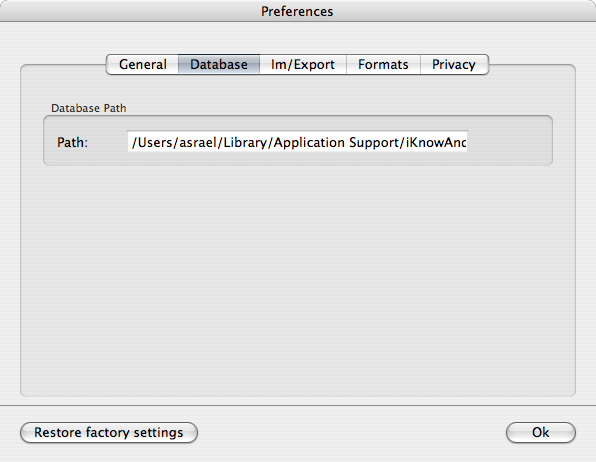
\includegraphics[width=13.5cm]{images/Prefs_Database.png}
\end{center}
\caption{Database Prefs}
\label{image:databaseprefs}
\end{figure}
\noindent
%
For the \textit{database} preferences there is currently not much (there is more to come). The only thing you can see here is where the system has its database file. This file is very important because it holds all information that is in the system. You can backup this file if you want to but currently you have to do this manually. For future releases a better handling of the database file is planed.
% ----------------------------------------------------------------------------------
\subsubsection{Im/Export}
\label{prefs_imexport}
\medskip
% 
\begin{figure}[ht]
\begin{center}
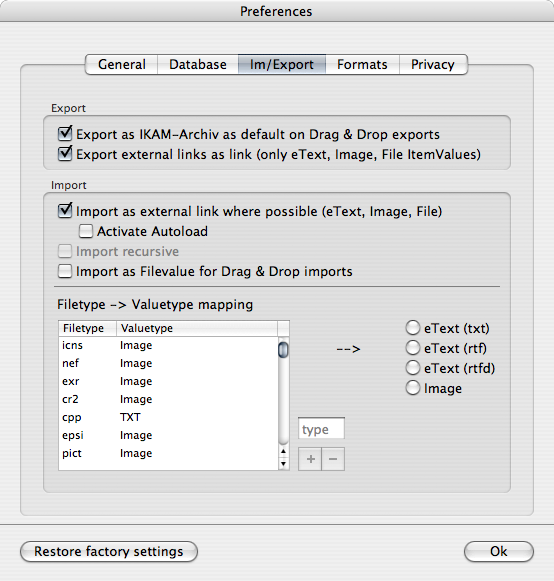
\includegraphics[width=13.5cm]{images/Prefs_ImExport.png}
\end{center}
\caption{Im/Export Prefs}
\label{image:imexportprefs}
\end{figure}
\noindent
%
The settings you can adjust here are (in figure \ref{image:imexportprefs}) mainly for Drag \& Drop im/export and they are taken as presets for the manual Im/Export dialogs (see chapter \ref{bring_data} and chapter \ref{export_data} for information on that). \\
We talked about most of the things you find here. What's now is the Filetype $\rightarrow$ Valuetype mapping. Since we have three Values which can have external links document, the system has to know without popping up a requester on Drag \& Drop what Valuetype you want to have created for which Filetype. For example, if you drag a .html file to iKnow \& Manage and you want to have a ExtendedText Value created for it then you should set the Filetype (.html/.htm) to "eText (txt)". If the Filetype does not exist you can create one with typing "html" into the \textit{type} text field and then hit the \textit{+} button. This will create a new Filetype $\rightarrow$ Valuetype mapping. You should now select the mapping and set "eText (txt)" for it as Valuetype.
% ----------------------------------------------------------------------------------
\subsubsection{Format}
\label{prefs_format}
\medskip
\textbf{Currency/Number:} \\
For all Number or Currency Values that you create you can choose the format in which they are shown on the screen. The setting currently is a global setting for all Values (see figure \ref{image:currencyprefs}). But it is planned to set format settings individually for Number/Currency and Date formats. \\
The options should be quite straight forward. The difference between Number and Currency is just the Currency Symbol that you can set. The settings for Currency and Number can be different. \\
\\
\textbf{Date:} \\
The display format for dates is build out of format characters which are shown and described in the "Available Formats" list (see figure \ref{image:dateprefs}). Select a format and the description is shown on the "Explanation" text view. You can build your own display format, just delete or add the format characters in the sequence you would like to have in the "Format:" text field. If you hit Enter, the date format is shown in the "Example" text field.
% 
\begin{figure}[ht]
\begin{center}
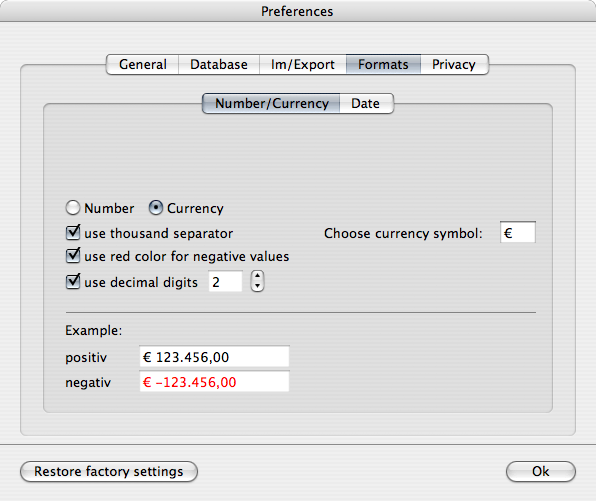
\includegraphics[width=13.5cm]{images/Prefs_CurrencyFormat.png}
\end{center}
\caption{Currency Prefs}
\label{image:currencyprefs}
\end{figure}
\noindent
%
% 
\begin{figure}[ht]
\begin{center}
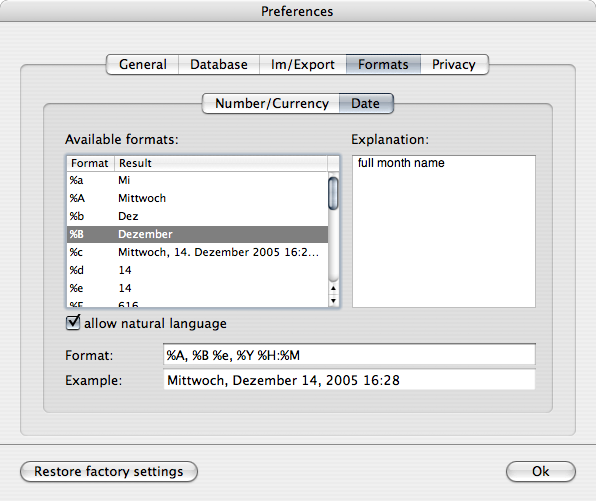
\includegraphics[width=13.5cm]{images/Prefs_DateFormat.png}
\end{center}
\caption{Date Prefs}
\label{image:dateprefs}
\end{figure}
\noindent
%
% ----------------------------------------------------------------------------------
\subsubsection{Privacy}
\label{prefs_privacy}
\medskip
There is not much at the privacy preferences (see figure \ref{image:privacyprefs}) right now but there is more to come. What you can do here is setting the default encryption password. After starting the first time there is no password set, so set one to use the "Encrypt with default password" function. If you want to alter the password, enter your old. When that fits, the text fields for entering the new password will be enabled. If you type twice the same password, the change button will be enabled and if you hit it, the new password will be set.
% 
\begin{figure}[ht]
\begin{center}
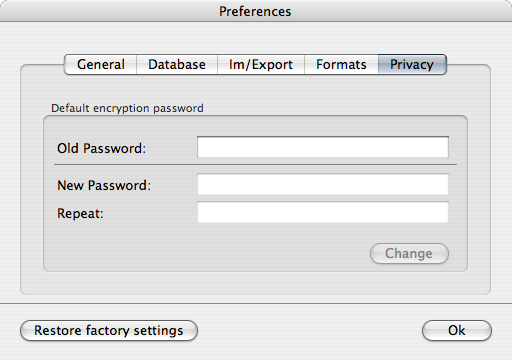
\includegraphics[width=13.5cm]{images/Prefs_Privacy.png}
\end{center}
\caption{Privacy Prefs}
\label{image:privacyprefs}
\end{figure}
\noindent
%
% ----------------------------------------------------------------------------------
% ----------------------------------------------------------------------------------
\clearpage
\newpage
\section{Printing}
\label{printing}
\medskip
There are two options for printing lists. \\
\\
% 
\begin{figure}[ht]
\begin{center}
\includegraphics[width=13.5cm]{images/Print_ItemValueDetail.png}
\end{center}
\caption{ItemValue Details}
\label{image:itemvalue_detail}
\end{figure}
\noindent
\textbf{Value detail lists:} \\
Detail lists show almost every information about the Value that is available. For Image Values only the thumbnail is shown, the text of RTF or RTFD is cropped to plain text. \\
To print detail lists just select all Values you want to have printed in the Value list view (see chapter \ref{gui_itemvaluelistview}) and choose "Print" from the main menu. You can select Values from different Items by selecting more Items at a time. All Values of the Item selection is shown in the table view. \\
See figure \ref{image:itemvalue_detail}. \\
\\
\textbf{ItemValue lists:} \\
To print a Item selection with all values of each Item just select the Items you want to have printed and choose "Print" from the main menu. See figure \ref{image:itemvalue_list}.
% 
\begin{figure}[ht]
\begin{center}
\includegraphics[width=13.5cm]{images/Print_ItemValueList.png}
\end{center}
\caption{ItemValue List}
\label{image:itemvalue_list}
\end{figure}
\noindent
% ----------------------------------------------------------------------------------
% ----------------------------------------------------------------------------------
\clearpage
\newpage
\section{Automatic updates}
\label{autoupdate}
\medskip
% 
\begin{figure}[ht]
\begin{center}
\includegraphics[width=13.5cm]{images/Update_Window.png}
\end{center}
\caption{Update Window}
\label{image:updates}
\end{figure}
\noindent
If you have activated the update checker in preferences to check on every startup and there is a new version available then a window will pop up informing you about the fact (see figure \ref{image:updates}). You can alternatively check manually through the main menu, choose "Help$\rightarrow$Check for Updates".
% ----------------------------------------------------------------------------------
% ----------------------------------------------------------------------------------
\newpage
\section{Registration}
\label{registration}
\medskip
% 
\begin{figure}[ht]
\begin{center}
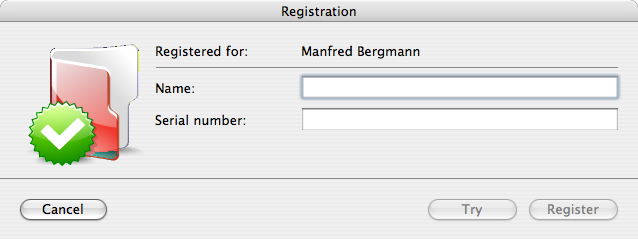
\includegraphics[width=13.5cm]{images/Registration_Window.png}
\end{center}
\caption{Registration Window}
\label{image:registration}
\end{figure}
\noindent
%
iKnow \& Manage is Shareware. If you decide to use it you have to pay for it. You can try this application for 30 days for free. A single user license costs US\$29.95. You can use the online registration form at Kagi. For European customers who do not have a credit card can transfer the money (EUR 29.95) directly on my bank account. But this way probably takes longer until you have the registration number and it means more work for me. There also may be a transaction fee if you are not in germany. \\
It can take one to seven days, depending on the method you have chosen, until I send the registration number.
\\
Kagi online registration form: \\
\href{http://order.kagi.com/?6FCEL}{http://order.kagi.com/?6FCEL} \\
\\
For using the bank transfer method more information is on the website: \\
\href{http://www.software-by-mabe.com/software/ikam.html#buy}{http://www.software-by-mabe.com/software/ikam.html\#buy}
% ----------------------------------------------------------------------------------
% ----------------------------------------------------------------------------------
\section{Disclaimer}
\label{disclaimer}
\medskip
software by MABE's applications are provided AS IS, without warranty of any kind, expressed or implied, including without limitation the warranties of merchantability, fitness for a particular purpose and non-infringement. The entire risk as to the quality and performance of software by MABE's applications is borne by you. Should software by MABE's applications prove defective, you and not software by MABE assume the entire cost of any service and repair. software by MABE is not responsible for any indirect, special, incidental, or consequential damages of any character including, but not limited to, damages for loss of goodwill, work stoppage, computer failure or malfunction, or any and all other commercial damages or losses.
% ----------------------------------------------------------------------------------
\end{document}

